
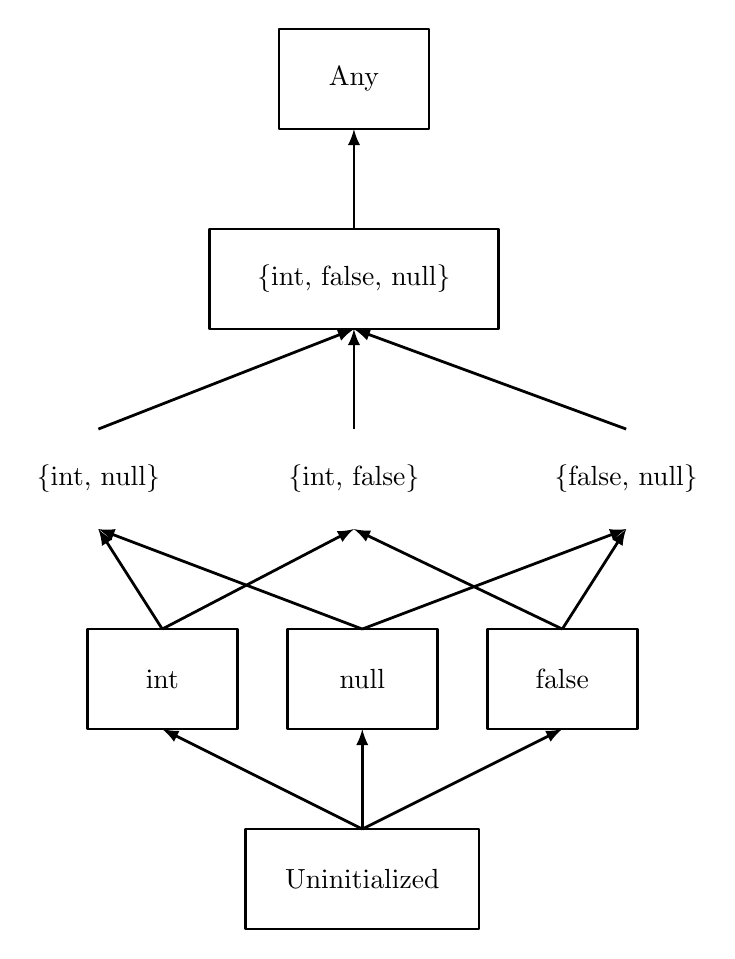
\begin{tikzpicture}[>=latex,line join=bevel,]
  \pgfsetlinewidth{1bp}
%%
\pgfsetcolor{black}
  % Edge: falsenull -> intfalsenull
  \draw [->] (225bp,180bp) .. controls (225bp,180bp) and (160.93bp,203.54bp)  .. (127bp,216bp);
  % Edge: intfalse -> intfalsenull
  \draw [->] (127bp,180bp) .. controls (127bp,180bp) and (127bp,195.14bp)  .. (127bp,216bp);
  % Edge: uninit -> null
  \draw [->] (130bp,36bp) .. controls (130bp,36bp) and (130bp,51.137bp)  .. (130bp,72bp);
  % Edge: int -> intnull
  \draw [->] (58bp,108bp) .. controls (58bp,108bp) and (47.375bp,124.63bp)  .. (35bp,144bp);
  % Edge: uninit -> int
  \draw [->] (130bp,36bp) .. controls (130bp,36bp) and (86.493bp,57.753bp)  .. (58bp,72bp);
  % Edge: false -> intfalse
  \draw [->] (202bp,108bp) .. controls (202bp,108bp) and (156.22bp,129.97bp)  .. (127bp,144bp);
  % Edge: intnull -> intfalsenull
  \draw [->] (35bp,180bp) .. controls (35bp,180bp) and (93.995bp,203.09bp)  .. (127bp,216bp);
  % Edge: null -> intnull
  \draw [->] (130bp,108bp) .. controls (130bp,108bp) and (68.485bp,131.31bp)  .. (35bp,144bp);
  % Edge: null -> falsenull
  \draw [->] (130bp,108bp) .. controls (130bp,108bp) and (191.51bp,131.31bp)  .. (225bp,144bp);
  % Edge: uninit -> false
  \draw [->] (130bp,36bp) .. controls (130bp,36bp) and (173.51bp,57.753bp)  .. (202bp,72bp);
  % Edge: intfalsenull -> any
  \draw [->] (127bp,252bp) .. controls (127bp,252bp) and (127bp,267.14bp)  .. (127bp,288bp);
  % Edge: false -> falsenull
  \draw [->] (202bp,108bp) .. controls (202bp,108bp) and (212.63bp,124.63bp)  .. (225bp,144bp);
  % Edge: int -> intfalse
  \draw [->] (58bp,108bp) .. controls (58bp,108bp) and (99.276bp,129.54bp)  .. (127bp,144bp);
  % Node: falsenull
\begin{scope}
  \definecolor{strokecol}{rgb}{0.0,0.0,0.0};
  \pgfsetstrokecolor{strokecol}
  \draw (225bp,162bp) node {\{false, null\}};
\end{scope}
  % Node: false
\begin{scope}
  \definecolor{strokecol}{rgb}{0.0,0.0,0.0};
  \pgfsetstrokecolor{strokecol}
  \draw (229bp,108bp) -- (175bp,108bp) -- (175bp,72bp) -- (229bp,72bp) -- cycle;
  \draw (202bp,90bp) node {false};
\end{scope}
  % Node: intfalsenull
\begin{scope}
  \definecolor{strokecol}{rgb}{0.0,0.0,0.0};
  \pgfsetstrokecolor{strokecol}
  \draw (179bp,252bp) -- (75bp,252bp) -- (75bp,216bp) -- (179bp,216bp) -- cycle;
  \draw (127bp,234bp) node {\{int, false, null\}};
\end{scope}
  % Node: int
\begin{scope}
  \definecolor{strokecol}{rgb}{0.0,0.0,0.0};
  \pgfsetstrokecolor{strokecol}
  \draw (85bp,108bp) -- (31bp,108bp) -- (31bp,72bp) -- (85bp,72bp) -- cycle;
  \draw (58bp,90bp) node {int};
\end{scope}
  % Node: uninit
\begin{scope}
  \definecolor{strokecol}{rgb}{0.0,0.0,0.0};
  \pgfsetstrokecolor{strokecol}
  \draw (172bp,36bp) -- (88bp,36bp) -- (88bp,0bp) -- (172bp,0bp) -- cycle;
  \draw (130bp,18bp) node {Uninitialized};
\end{scope}
  % Node: intnull
\begin{scope}
  \definecolor{strokecol}{rgb}{0.0,0.0,0.0};
  \pgfsetstrokecolor{strokecol}
  \draw (35bp,162bp) node {\{int, null\}};
\end{scope}
  % Node: intfalse
\begin{scope}
  \definecolor{strokecol}{rgb}{0.0,0.0,0.0};
  \pgfsetstrokecolor{strokecol}
  \draw (127bp,162bp) node {\{int, false\}};
\end{scope}
  % Node: null
\begin{scope}
  \definecolor{strokecol}{rgb}{0.0,0.0,0.0};
  \pgfsetstrokecolor{strokecol}
  \draw (157bp,108bp) -- (103bp,108bp) -- (103bp,72bp) -- (157bp,72bp) -- cycle;
  \draw (130bp,90bp) node {null};
\end{scope}
  % Node: any
\begin{scope}
  \definecolor{strokecol}{rgb}{0.0,0.0,0.0};
  \pgfsetstrokecolor{strokecol}
  \draw (154bp,324bp) -- (100bp,324bp) -- (100bp,288bp) -- (154bp,288bp) -- cycle;
  \draw (127bp,306bp) node {Any};
\end{scope}
%
\end{tikzpicture}

